\documentclass[a4paper, fontsize=11pt]{scrartcl} % A4 paper and 11pt font 
\usepackage[a4paper,left=3cm,right=2cm,top=2.5cm,bottom=2.5cm]{geometry}

\usepackage[T1]{fontenc} % Use 8-bit encoding that has 256 glyphs
\usepackage{fourier} % Use the Adobe Utopia font for the document - comment this line to return to the LaTeX default
\usepackage[spanish]{babel} % Spanish language/hyphenation
\selectlanguage{spanish}
\usepackage[utf8]{inputenc}
\usepackage{amsmath,amsfonts,amsthm} % Math packages
\usepackage{graphicx} % The graphicx package
\usepackage{placeins}
\usepackage{caption}
\usepackage{subcaption}


\usepackage{listings} % Insert Scripts
\usepackage{color} %red, green, blue, yellow, cyan, magenta, black, white
\definecolor{mygreen}{RGB}{28,172,0} % color values Red, Green, Blue
\definecolor{mylilas}{RGB}{170,55,241}

\lstset{language=Matlab,%
	%basicstyle=\color{red},
	breaklines=true,%
	morekeywords={matlab2tikz},
	keywordstyle=\color{blue},%
	morekeywords=[2]{1}, keywordstyle=[2]{\color{black}},
	identifierstyle=\color{black},%
	stringstyle=\color{mylilas},
	commentstyle=\color{mygreen},%
	showstringspaces=false,%without this there will be a symbol in the places where there is a space
	numbers=left,%
	numberstyle={\tiny \color{black}},% size of the numbers
	numbersep=9pt, % this defines how far the numbers are from the text
	emph=[1]{for,end,break},emphstyle=[1]\color{red}, %some words to emphasise
	%emph=[2]{word1,word2}, emphstyle=[2]{style},    
}

\usepackage{sectsty} % Allows customizing section commands
%\allsectionsfont{\centering \normalfont\scshape} % Make all sections centered, the default font and small caps

\usepackage{fancyhdr} % Custom headers and footers
\pagestyle{fancyplain} % Makes all pages in the document conform to the custom headers and footers
\fancyhead{} % No page header - if you want one, create it in the same way as the footers below
\fancyfoot[L]{} % Empty left footer
\fancyfoot[C]{} % Empty center footer
\fancyfoot[R]{\thepage} % Page numbering for right footer
\renewcommand{\headrulewidth}{0pt} % Remove header underlines
\renewcommand{\footrulewidth}{0pt} % Remove footer underlines
\setlength{\headheight}{13.6pt} % Customize the height of the header

\numberwithin{equation}{section} % Number equations within sections (i.e. 1.1, 1.2, 2.1, 2.2 instead of 1, 2, 3, 4)
\numberwithin{figure}{section} % Number figures within sections (i.e. 1.1, 1.2, 2.1, 2.2 instead of 1, 2, 3, 4)
\numberwithin{table}{section} % Number tables within sections (i.e. 1.1, 1.2, 2.1, 2.2 instead of 1, 2, 3, 4)

%\setlength\parindent{0pt} % Removes all indentation from paragraphs - comment this line for an assignment with lots of text

\newenvironment{myalign}{\par\nobreak\large\noindent\align}{\endalign} %Altering fontsize in equations globally

%----------------------------------------------------------------------------------------
%	TITLE SECTION
%----------------------------------------------------------------------------------------

\newcommand{\horrule}[1]{\rule{\linewidth}{#1}} % Create horizontal rule command with 1 argument of height

\title{	
	\normalfont \normalsize 
	\textsc{Master en Automática y Robótica - UPM} \\ [25pt] % Your university, school and/or department name(s)
	\horrule{0.5pt} \\[0.4cm] % Thin top horizontal rule
	\huge Control de Mínima Varianza \\ % The assignment title
	\horrule{2pt} \\[0.5cm] % Thick bottom horizontal rule
}

\author{Jorge Camarero Vera - 07052} % Your name

\date{\normalsize\today} % Today's date or a custom date

\begin{document}
	\maketitle
	
	\section{Explicación de la tarea}
	
	La finalidad de esta tarea es implementar un regulador predictivo en el \textit{sistema\_tema\_3y4}, el cuál permita minimizar la varianza de salida. El modelo \textit{sistema\_tema\_3y4} tiene sus bloques identificados en trabajos anteriores, con ruido de entrada de $\sigma^2 = 0.6$,  por lo que en esta tarea las funciones de transferencia están identificadas, Figura \ref{Modelo Inicial}.\\
	
	\begin{figure}[h!]
		\centering
		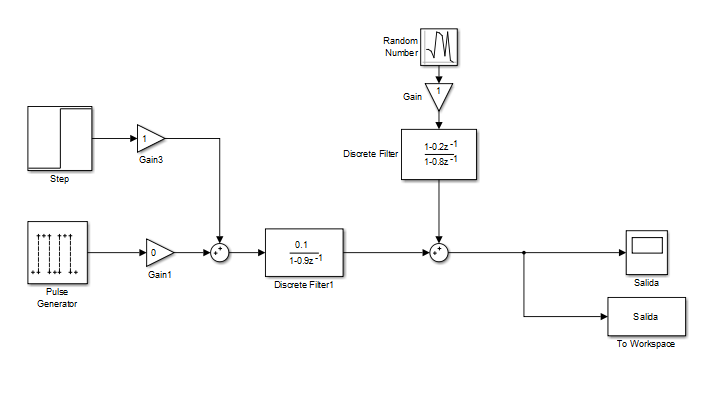
\includegraphics[width=1.0\linewidth]{images/Original_System.PNG}
		\caption{Modelo inicial}
		\label{Modelo Inicial}
	\end{figure}
	\FloatBarrier
	
	\subsection{Presentación de los datos}
	
	Los valores de la señal de salida ante entrada escalón con valor de $80$ son los de la Figura \ref{Salida}. Filtrando los datos iniciales se quedan en los de la Figura \ref{SalidaP}.
	
	\begin{figure}[h!]
		\centering
		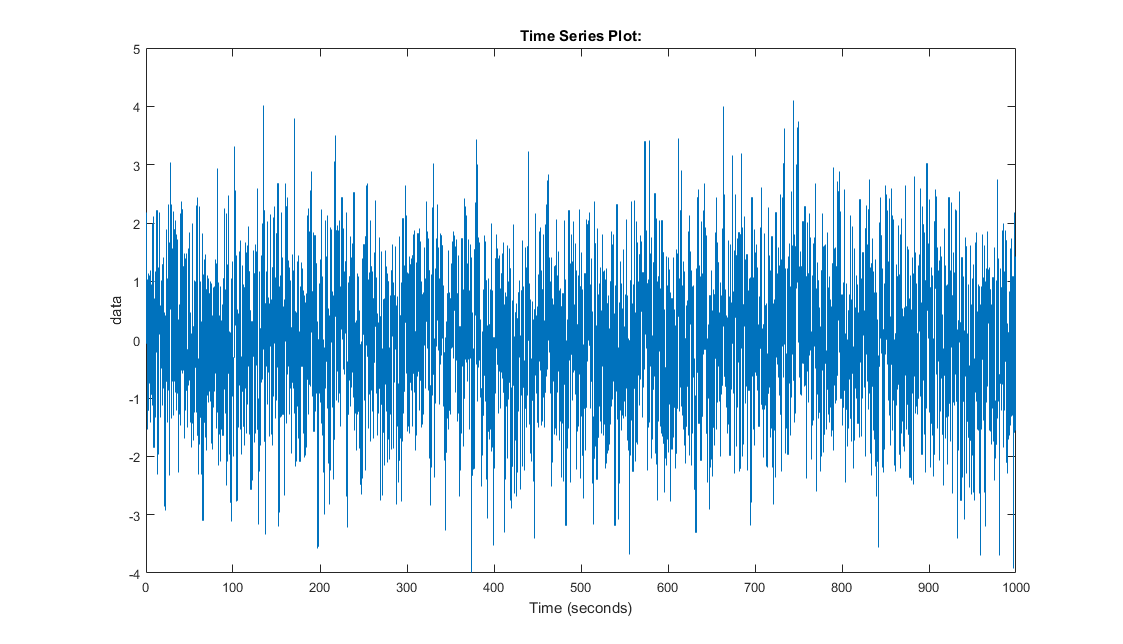
\includegraphics[width=1.0\linewidth]{images/output.PNG}
		\caption{Salida del Sistema}
		\label{Salida}
	\end{figure}
	\FloatBarrier
	
	\begin{figure}[h!]
		\centering
		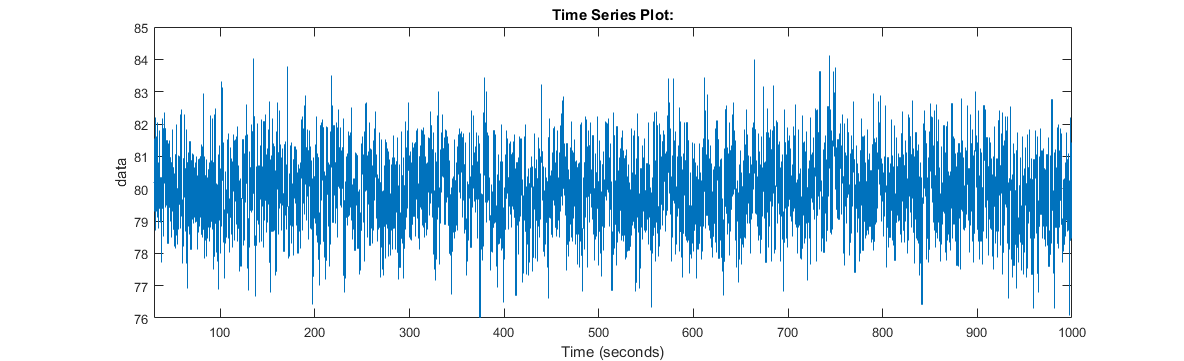
\includegraphics[width=1.0\linewidth]{images/outputP.PNG}
		\caption{Salida del Sistema, filtrados los 30 primeros valores.}
		\label{SalidaP}
	\end{figure}
	\FloatBarrier
	
	La varianza de estos últimos valores es:
	
	\begin{lstlisting}
	>> variance1 = var(Salida.Data(30:end))
	
	variance1 =
	
	1.2256 
	\end{lstlisting}
	
	\begin{myalign}
		\sigma = 1.2256
		\label{varOr}
	\end{myalign}

	\section{Regulador de Mínima Varianza}	
	
	El sistema de la Figura \ref{Modelo Inicial} se puede modelar como un ARMAX, es análogo al modelo ARMA, pero con una entrada auxiliar.
	
	\begin{myalign}
		A(z^{-1})Y(z)=B(z^{-1})U(z)+C(z^{-1})w(z)\\
	\end{myalign}
	
	Siendo $w(k) \rightarrow N(0,\sigma)$.\\
	
	La regulación de mínima varianza consiste en predecir con cierta antelación la componente estocástica $n(k)$. Para a continuación pasar a su neutralización a través de la acción de la componente determinista $v(k)$. Se trata de efectuar un control u(k) en el instante actual, para que $d$ instantes más tarde, $v(k)$ neutralice la perturbación $n(k)$.\\
	
	\begin{figure}[h!]
		\centering
		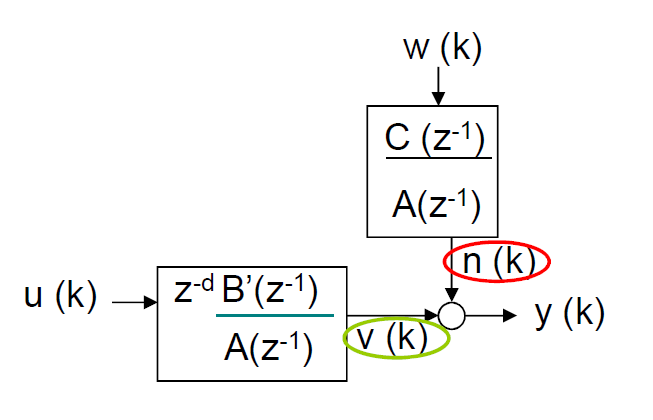
\includegraphics[width=0.6\linewidth]{images/Regulation.PNG}
		\caption{Planteamiento del problema}
		\label{Regulation}
	\end{figure}
	\FloatBarrier
	
	Para mejorar la predicción del sistema debemos de reducir la varianza. Para ello planteamos el sistema como en la Figura \ref{Regulator}.
	
	\begin{figure}[h!]
		\centering
		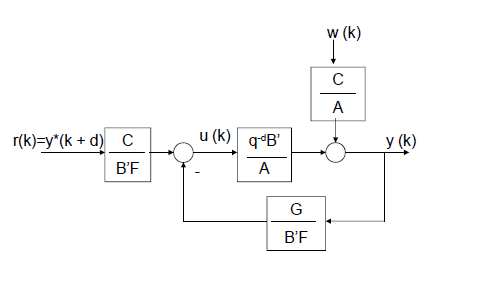
\includegraphics[width=1.0\linewidth]{images/Regulator.PNG}
		\caption{Regulador predictivo}
		\label{Regulator}
	\end{figure}
	\FloatBarrier
	
	Si alguna raíz de $C(z)$ o de $B'(z)F(z)$ está sobre o fuera de la circunferencia unidad, el sistema sería \textbf{inestable} y no se podría aplicar el regulador propuesto.\\
	
	Calculamos:
	
	\begin{lstlisting}
		A = conv(poly(0.9), poly(0.8))
		C = conv(poly(0.2), poly(0.9))
		Bp = poly(0.8)
		
		A =
		
		1.0000   -1.7000    0.7200
		
		
		C =
		
		1.0000   -1.1000    0.1800
		
		
		Bp =
		
		1.0000   -0.8000
		
	\end{lstlisting}
	
	\begin{myalign}
		\begin{split}
			&A(z^{-1}) = (1 - 0.9z^{-1})(1 - 0.8z^{-1})= 1 - 1.7z^{-1} + 0.72z^{-2}\\
			&C(z^{-1}) = (1 - 0.2z^{-1})(1 - 0.9z^{-1}) = 1 - 1.1z^{-1} + 0.18z^{-2}\\
			&B'(z^{-1}) = 1 - 0.8z^{-1}
		\end{split}		
	\end{myalign}
	
	\begin{lstlisting}
		>> [F G] = deconv(C,A)
		
		F =
		
		1
		
		
		G =
		
		0    0.6000   -0.5400
	\end{lstlisting}
	
	\begin{myalign}
		\begin{split}
			&F(z^{-1}) = 1\\
			&G(z^{-1}) = 0.6 - 0.54z^{-1}
		\end{split}
	\end{myalign}
	
	Teniendo $C(z^{-1})$, $B'(z^{-1})$ $F(z^{-1})$ y $G(z^{-1})$, podemos completar nuestro regulador, Figura \ref{Final}.
	
	\begin{figure}[h!]
		\centering
		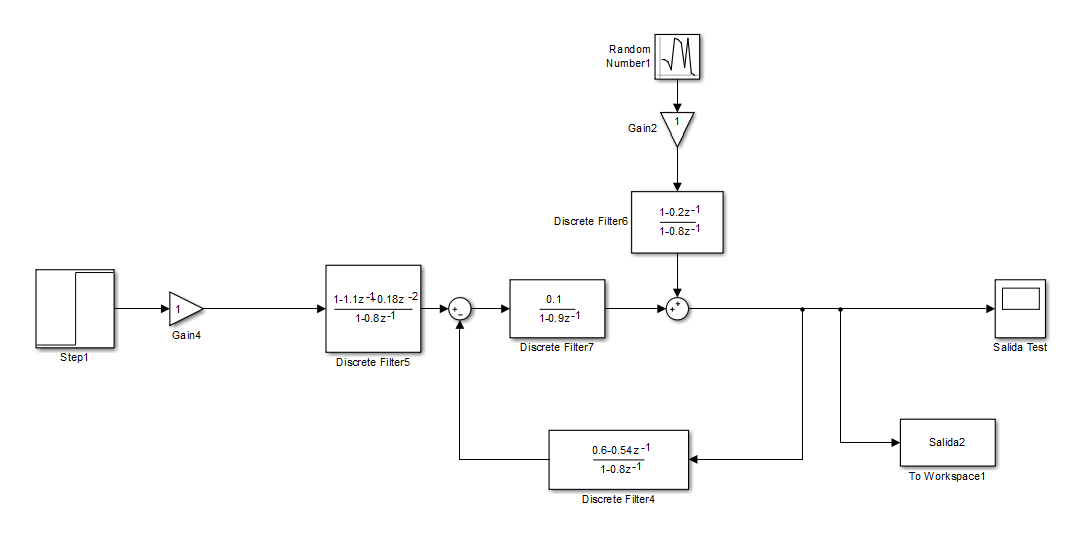
\includegraphics[width=1.0\linewidth]{images/FinalModel.PNG}
		\caption{Sistema con regulador predictivo de mínima varianza}
		\label{Final}
	\end{figure}
	\FloatBarrier
	
	La salida de este sistema filtrando los 30 primeros valores es la Figura \ref{Salida2}.
	
	\begin{figure}[h!]
		\centering
		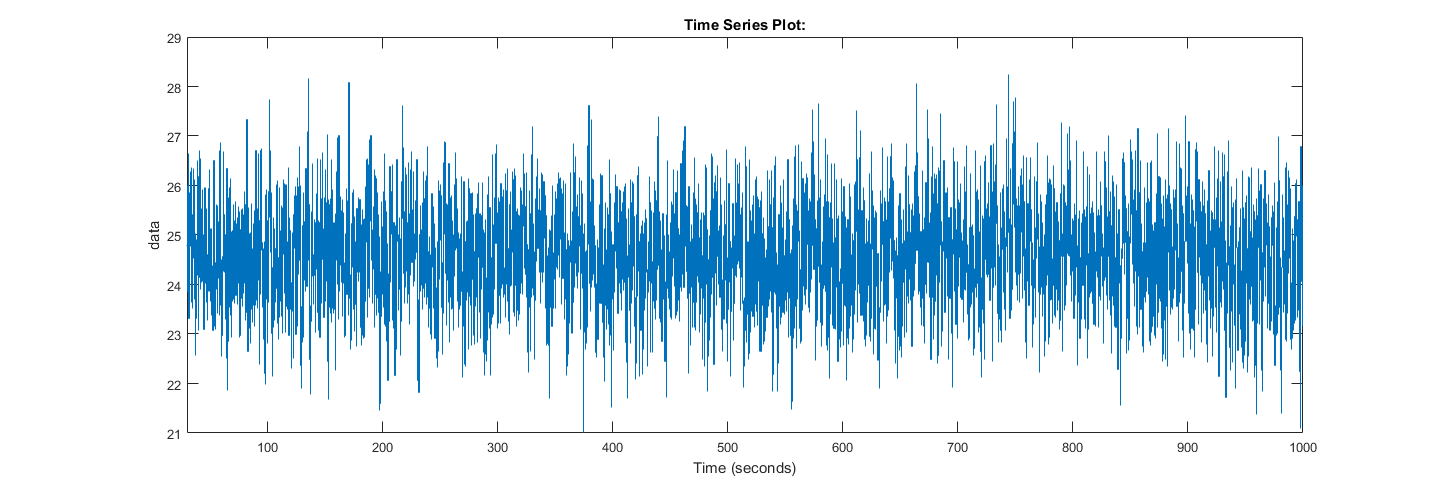
\includegraphics[width=1.0\linewidth]{images/output2.PNG}
		\caption{Salida de mínima varianza}
		\label{Salida2}
	\end{figure}
	\FloatBarrier
	
	Con una varianza de:
	
	\begin{lstlisting}
		>> variance2 = var(Salida2.Data(30:end))
		
		variance2 =
		
		0.9024
	\end{lstlisting}
	
	\begin{myalign}
		\sigma = 0.9024
		\label{varReg}
	\end{myalign}
	
	Vemos que esta \textbf{varianza (\ref{varReg}) es menor a la original (\ref{varOr})}, por lo que hemos comprobado que el regulador creado reduce la varianza de salida, pero el valor medio de los valores en ambas salidas es muy distinto, la original tiene una media de $80$, mientras que la regulada tiene una media de $24.6$, por lo que se habrá de intentar regular el error de referencia.
	
\end{document}